% Created by tikzDevice version 0.12.3.1 on 2022-05-04 14:00:27
% !TEX encoding = UTF-8 Unicode
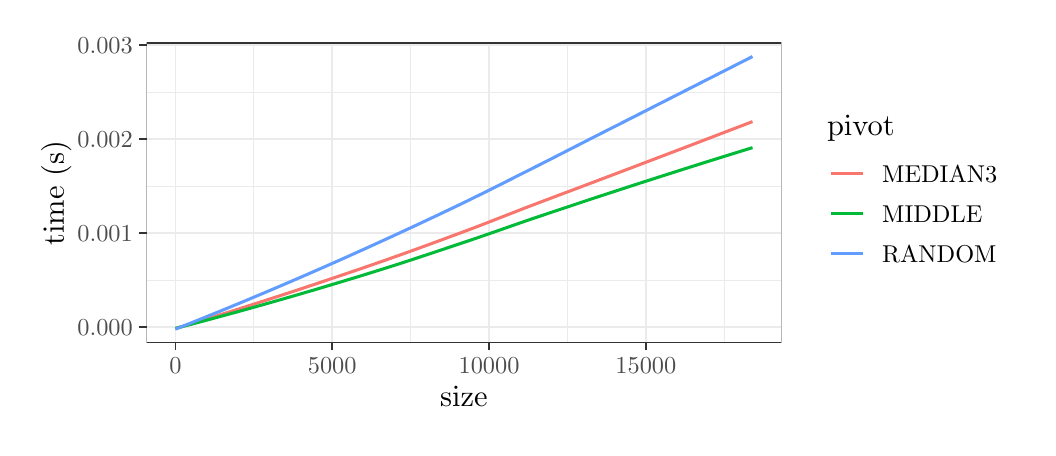
\begin{tikzpicture}[x=1pt,y=1pt]
\definecolor{fillColor}{RGB}{255,255,255}
\path[use as bounding box,fill=fillColor,fill opacity=0.00] (0,0) rectangle (361.35,144.54);
\begin{scope}
\path[clip] (  0.00,  0.00) rectangle (361.35,144.54);
\definecolor{drawColor}{RGB}{255,255,255}
\definecolor{fillColor}{RGB}{255,255,255}

\path[draw=drawColor,line width= 0.6pt,line join=round,line cap=round,fill=fillColor] (  0.00,  0.00) rectangle (361.35,144.54);
\end{scope}
\begin{scope}
\path[clip] ( 42.95, 30.69) rectangle (272.35,139.04);
\definecolor{fillColor}{RGB}{255,255,255}

\path[fill=fillColor] ( 42.95, 30.69) rectangle (272.35,139.04);
\definecolor{drawColor}{gray}{0.92}

\path[draw=drawColor,line width= 0.3pt,line join=round] ( 42.95, 53.31) --
	(272.35, 53.31);

\path[draw=drawColor,line width= 0.3pt,line join=round] ( 42.95, 87.29) --
	(272.35, 87.29);

\path[draw=drawColor,line width= 0.3pt,line join=round] ( 42.95,121.27) --
	(272.35,121.27);

\path[draw=drawColor,line width= 0.3pt,line join=round] ( 81.72, 30.69) --
	( 81.72,139.04);

\path[draw=drawColor,line width= 0.3pt,line join=round] (138.38, 30.69) --
	(138.38,139.04);

\path[draw=drawColor,line width= 0.3pt,line join=round] (195.05, 30.69) --
	(195.05,139.04);

\path[draw=drawColor,line width= 0.3pt,line join=round] (251.72, 30.69) --
	(251.72,139.04);

\path[draw=drawColor,line width= 0.6pt,line join=round] ( 42.95, 36.32) --
	(272.35, 36.32);

\path[draw=drawColor,line width= 0.6pt,line join=round] ( 42.95, 70.30) --
	(272.35, 70.30);

\path[draw=drawColor,line width= 0.6pt,line join=round] ( 42.95,104.28) --
	(272.35,104.28);

\path[draw=drawColor,line width= 0.6pt,line join=round] ( 42.95,138.26) --
	(272.35,138.26);

\path[draw=drawColor,line width= 0.6pt,line join=round] ( 53.38, 30.69) --
	( 53.38,139.04);

\path[draw=drawColor,line width= 0.6pt,line join=round] (110.05, 30.69) --
	(110.05,139.04);

\path[draw=drawColor,line width= 0.6pt,line join=round] (166.72, 30.69) --
	(166.72,139.04);

\path[draw=drawColor,line width= 0.6pt,line join=round] (223.39, 30.69) --
	(223.39,139.04);
\definecolor{drawColor}{RGB}{248,118,109}

\path[draw=drawColor,line width= 1.1pt,line join=round] ( 53.38, 35.82) --
	( 56.02, 36.62) --
	( 58.66, 37.42) --
	( 61.30, 38.23) --
	( 63.94, 39.05) --
	( 66.58, 39.86) --
	( 69.22, 40.69) --
	( 71.86, 41.51) --
	( 74.50, 42.34) --
	( 77.14, 43.18) --
	( 79.78, 44.02) --
	( 82.42, 44.86) --
	( 85.06, 45.71) --
	( 87.70, 46.56) --
	( 90.34, 47.41) --
	( 92.98, 48.27) --
	( 95.62, 49.13) --
	( 98.26, 50.00) --
	(100.90, 50.88) --
	(103.54, 51.75) --
	(106.18, 52.64) --
	(108.82, 53.53) --
	(111.46, 54.42) --
	(114.10, 55.31) --
	(116.74, 56.21) --
	(119.38, 57.11) --
	(122.02, 58.01) --
	(124.65, 58.92) --
	(127.29, 59.84) --
	(129.93, 60.77) --
	(132.57, 61.70) --
	(135.21, 62.64) --
	(137.85, 63.58) --
	(140.49, 64.54) --
	(143.13, 65.50) --
	(145.77, 66.46) --
	(148.41, 67.43) --
	(151.05, 68.41) --
	(153.69, 69.39) --
	(156.33, 70.36) --
	(158.97, 71.35) --
	(161.61, 72.34) --
	(164.25, 73.35) --
	(166.89, 74.38) --
	(169.53, 75.41) --
	(172.17, 76.44) --
	(174.81, 77.47) --
	(177.45, 78.50) --
	(180.09, 79.53) --
	(182.73, 80.54) --
	(185.37, 81.54) --
	(188.01, 82.53) --
	(190.65, 83.53) --
	(193.29, 84.52) --
	(195.93, 85.51) --
	(198.57, 86.50) --
	(201.21, 87.50) --
	(203.85, 88.49) --
	(206.49, 89.49) --
	(209.13, 90.49) --
	(211.77, 91.49) --
	(214.41, 92.49) --
	(217.05, 93.49) --
	(219.69, 94.49) --
	(222.33, 95.49) --
	(224.97, 96.50) --
	(227.61, 97.50) --
	(230.25, 98.50) --
	(232.89, 99.51) --
	(235.53,100.51) --
	(238.17,101.52) --
	(240.81,102.52) --
	(243.44,103.53) --
	(246.08,104.54) --
	(248.72,105.55) --
	(251.36,106.56) --
	(254.00,107.57) --
	(256.64,108.58) --
	(259.28,109.59) --
	(261.92,110.60);
\definecolor{drawColor}{RGB}{0,186,56}

\path[draw=drawColor,line width= 1.1pt,line join=round] ( 53.38, 35.88) --
	( 56.02, 36.56) --
	( 58.66, 37.25) --
	( 61.30, 37.95) --
	( 63.94, 38.65) --
	( 66.58, 39.36) --
	( 69.22, 40.07) --
	( 71.86, 40.79) --
	( 74.50, 41.51) --
	( 77.14, 42.24) --
	( 79.78, 42.97) --
	( 82.42, 43.71) --
	( 85.06, 44.45) --
	( 87.70, 45.20) --
	( 90.34, 45.95) --
	( 92.98, 46.71) --
	( 95.62, 47.47) --
	( 98.26, 48.23) --
	(100.90, 49.01) --
	(103.54, 49.78) --
	(106.18, 50.57) --
	(108.82, 51.36) --
	(111.46, 52.15) --
	(114.10, 52.95) --
	(116.74, 53.75) --
	(119.38, 54.55) --
	(122.02, 55.37) --
	(124.65, 56.18) --
	(127.29, 57.01) --
	(129.93, 57.84) --
	(132.57, 58.67) --
	(135.21, 59.52) --
	(137.85, 60.38) --
	(140.49, 61.24) --
	(143.13, 62.12) --
	(145.77, 62.99) --
	(148.41, 63.87) --
	(151.05, 64.76) --
	(153.69, 65.64) --
	(156.33, 66.52) --
	(158.97, 67.40) --
	(161.61, 68.30) --
	(164.25, 69.21) --
	(166.89, 70.12) --
	(169.53, 71.04) --
	(172.17, 71.97) --
	(174.81, 72.89) --
	(177.45, 73.81) --
	(180.09, 74.73) --
	(182.73, 75.63) --
	(185.37, 76.51) --
	(188.01, 77.40) --
	(190.65, 78.28) --
	(193.29, 79.17) --
	(195.93, 80.05) --
	(198.57, 80.93) --
	(201.21, 81.80) --
	(203.85, 82.68) --
	(206.49, 83.55) --
	(209.13, 84.41) --
	(211.77, 85.28) --
	(214.41, 86.14) --
	(217.05, 87.00) --
	(219.69, 87.85) --
	(222.33, 88.71) --
	(224.97, 89.56) --
	(227.61, 90.41) --
	(230.25, 91.25) --
	(232.89, 92.09) --
	(235.53, 92.93) --
	(238.17, 93.77) --
	(240.81, 94.61) --
	(243.44, 95.44) --
	(246.08, 96.27) --
	(248.72, 97.09) --
	(251.36, 97.92) --
	(254.00, 98.74) --
	(256.64, 99.56) --
	(259.28,100.38) --
	(261.92,101.19);
\definecolor{drawColor}{RGB}{97,156,255}

\path[draw=drawColor,line width= 1.1pt,line join=round] ( 53.38, 35.61) --
	( 56.02, 36.66) --
	( 58.66, 37.71) --
	( 61.30, 38.77) --
	( 63.94, 39.83) --
	( 66.58, 40.90) --
	( 69.22, 41.97) --
	( 71.86, 43.05) --
	( 74.50, 44.14) --
	( 77.14, 45.23) --
	( 79.78, 46.33) --
	( 82.42, 47.44) --
	( 85.06, 48.55) --
	( 87.70, 49.66) --
	( 90.34, 50.79) --
	( 92.98, 51.91) --
	( 95.62, 53.05) --
	( 98.26, 54.19) --
	(100.90, 55.33) --
	(103.54, 56.49) --
	(106.18, 57.64) --
	(108.82, 58.81) --
	(111.46, 59.97) --
	(114.10, 61.15) --
	(116.74, 62.33) --
	(119.38, 63.52) --
	(122.02, 64.71) --
	(124.65, 65.91) --
	(127.29, 67.11) --
	(129.93, 68.32) --
	(132.57, 69.53) --
	(135.21, 70.75) --
	(137.85, 71.97) --
	(140.49, 73.20) --
	(143.13, 74.44) --
	(145.77, 75.68) --
	(148.41, 76.92) --
	(151.05, 78.18) --
	(153.69, 79.44) --
	(156.33, 80.71) --
	(158.97, 81.98) --
	(161.61, 83.28) --
	(164.25, 84.58) --
	(166.89, 85.89) --
	(169.53, 87.21) --
	(172.17, 88.54) --
	(174.81, 89.87) --
	(177.45, 91.21) --
	(180.09, 92.54) --
	(182.73, 93.87) --
	(185.37, 95.20) --
	(188.01, 96.54) --
	(190.65, 97.88) --
	(193.29, 99.23) --
	(195.93,100.58) --
	(198.57,101.93) --
	(201.21,103.28) --
	(203.85,104.63) --
	(206.49,105.97) --
	(209.13,107.31) --
	(211.77,108.65) --
	(214.41,109.98) --
	(217.05,111.32) --
	(219.69,112.66) --
	(222.33,114.00) --
	(224.97,115.35) --
	(227.61,116.69) --
	(230.25,118.03) --
	(232.89,119.37) --
	(235.53,120.71) --
	(238.17,122.05) --
	(240.81,123.39) --
	(243.44,124.73) --
	(246.08,126.07) --
	(248.72,127.41) --
	(251.36,128.75) --
	(254.00,130.09) --
	(256.64,131.43) --
	(259.28,132.77) --
	(261.92,134.11);
\definecolor{drawColor}{gray}{0.20}

\path[draw=drawColor,line width= 0.6pt,line join=round,line cap=round] ( 42.95, 30.69) rectangle (272.35,139.04);
\end{scope}
\begin{scope}
\path[clip] (  0.00,  0.00) rectangle (361.35,144.54);
\definecolor{drawColor}{gray}{0.30}

\node[text=drawColor,anchor=base east,inner sep=0pt, outer sep=0pt, scale=  0.88] at ( 38.00, 33.29) {0.000};

\node[text=drawColor,anchor=base east,inner sep=0pt, outer sep=0pt, scale=  0.88] at ( 38.00, 67.27) {0.001};

\node[text=drawColor,anchor=base east,inner sep=0pt, outer sep=0pt, scale=  0.88] at ( 38.00,101.25) {0.002};

\node[text=drawColor,anchor=base east,inner sep=0pt, outer sep=0pt, scale=  0.88] at ( 38.00,135.23) {0.003};
\end{scope}
\begin{scope}
\path[clip] (  0.00,  0.00) rectangle (361.35,144.54);
\definecolor{drawColor}{gray}{0.20}

\path[draw=drawColor,line width= 0.6pt,line join=round] ( 40.20, 36.32) --
	( 42.95, 36.32);

\path[draw=drawColor,line width= 0.6pt,line join=round] ( 40.20, 70.30) --
	( 42.95, 70.30);

\path[draw=drawColor,line width= 0.6pt,line join=round] ( 40.20,104.28) --
	( 42.95,104.28);

\path[draw=drawColor,line width= 0.6pt,line join=round] ( 40.20,138.26) --
	( 42.95,138.26);
\end{scope}
\begin{scope}
\path[clip] (  0.00,  0.00) rectangle (361.35,144.54);
\definecolor{drawColor}{gray}{0.20}

\path[draw=drawColor,line width= 0.6pt,line join=round] ( 53.38, 27.94) --
	( 53.38, 30.69);

\path[draw=drawColor,line width= 0.6pt,line join=round] (110.05, 27.94) --
	(110.05, 30.69);

\path[draw=drawColor,line width= 0.6pt,line join=round] (166.72, 27.94) --
	(166.72, 30.69);

\path[draw=drawColor,line width= 0.6pt,line join=round] (223.39, 27.94) --
	(223.39, 30.69);
\end{scope}
\begin{scope}
\path[clip] (  0.00,  0.00) rectangle (361.35,144.54);
\definecolor{drawColor}{gray}{0.30}

\node[text=drawColor,anchor=base,inner sep=0pt, outer sep=0pt, scale=  0.88] at ( 53.38, 19.68) {0};

\node[text=drawColor,anchor=base,inner sep=0pt, outer sep=0pt, scale=  0.88] at (110.05, 19.68) {5000};

\node[text=drawColor,anchor=base,inner sep=0pt, outer sep=0pt, scale=  0.88] at (166.72, 19.68) {10000};

\node[text=drawColor,anchor=base,inner sep=0pt, outer sep=0pt, scale=  0.88] at (223.39, 19.68) {15000};
\end{scope}
\begin{scope}
\path[clip] (  0.00,  0.00) rectangle (361.35,144.54);
\definecolor{drawColor}{RGB}{0,0,0}

\node[text=drawColor,anchor=base,inner sep=0pt, outer sep=0pt, scale=  1.10] at (157.65,  7.64) {size};
\end{scope}
\begin{scope}
\path[clip] (  0.00,  0.00) rectangle (361.35,144.54);
\definecolor{drawColor}{RGB}{0,0,0}

\node[text=drawColor,rotate= 90.00,anchor=base,inner sep=0pt, outer sep=0pt, scale=  1.10] at ( 13.08, 84.86) {time (s)};
\end{scope}
\begin{scope}
\path[clip] (  0.00,  0.00) rectangle (361.35,144.54);
\definecolor{fillColor}{RGB}{255,255,255}

\path[fill=fillColor] (283.35, 50.07) rectangle (355.85,119.65);
\end{scope}
\begin{scope}
\path[clip] (  0.00,  0.00) rectangle (361.35,144.54);
\definecolor{drawColor}{RGB}{0,0,0}

\node[text=drawColor,anchor=base west,inner sep=0pt, outer sep=0pt, scale=  1.10] at (288.85,105.51) {pivot};
\end{scope}
\begin{scope}
\path[clip] (  0.00,  0.00) rectangle (361.35,144.54);
\definecolor{fillColor}{RGB}{255,255,255}

\path[fill=fillColor] (288.85, 84.48) rectangle (303.30, 98.94);
\end{scope}
\begin{scope}
\path[clip] (  0.00,  0.00) rectangle (361.35,144.54);
\definecolor{drawColor}{RGB}{248,118,109}

\path[draw=drawColor,line width= 1.1pt,line join=round] (290.30, 91.71) -- (301.86, 91.71);
\end{scope}
\begin{scope}
\path[clip] (  0.00,  0.00) rectangle (361.35,144.54);
\definecolor{fillColor}{RGB}{255,255,255}

\path[fill=fillColor] (288.85, 70.03) rectangle (303.30, 84.48);
\end{scope}
\begin{scope}
\path[clip] (  0.00,  0.00) rectangle (361.35,144.54);
\definecolor{drawColor}{RGB}{0,186,56}

\path[draw=drawColor,line width= 1.1pt,line join=round] (290.30, 77.26) -- (301.86, 77.26);
\end{scope}
\begin{scope}
\path[clip] (  0.00,  0.00) rectangle (361.35,144.54);
\definecolor{fillColor}{RGB}{255,255,255}

\path[fill=fillColor] (288.85, 55.57) rectangle (303.30, 70.03);
\end{scope}
\begin{scope}
\path[clip] (  0.00,  0.00) rectangle (361.35,144.54);
\definecolor{drawColor}{RGB}{97,156,255}

\path[draw=drawColor,line width= 1.1pt,line join=round] (290.30, 62.80) -- (301.86, 62.80);
\end{scope}
\begin{scope}
\path[clip] (  0.00,  0.00) rectangle (361.35,144.54);
\definecolor{drawColor}{RGB}{0,0,0}

\node[text=drawColor,anchor=base west,inner sep=0pt, outer sep=0pt, scale=  0.88] at (308.80, 88.68) {MEDIAN3};
\end{scope}
\begin{scope}
\path[clip] (  0.00,  0.00) rectangle (361.35,144.54);
\definecolor{drawColor}{RGB}{0,0,0}

\node[text=drawColor,anchor=base west,inner sep=0pt, outer sep=0pt, scale=  0.88] at (308.80, 74.23) {MIDDLE};
\end{scope}
\begin{scope}
\path[clip] (  0.00,  0.00) rectangle (361.35,144.54);
\definecolor{drawColor}{RGB}{0,0,0}

\node[text=drawColor,anchor=base west,inner sep=0pt, outer sep=0pt, scale=  0.88] at (308.80, 59.77) {RANDOM};
\end{scope}
\end{tikzpicture}
